\documentclass[a4paper]{article}
%-----------------------------------------------------------------------------%
\usepackage{graphicx}
\usepackage{verbatim}
%-----------------------------------------------------------------------------%

\begin{document}

\begin{figure}[t!]
	\centering
	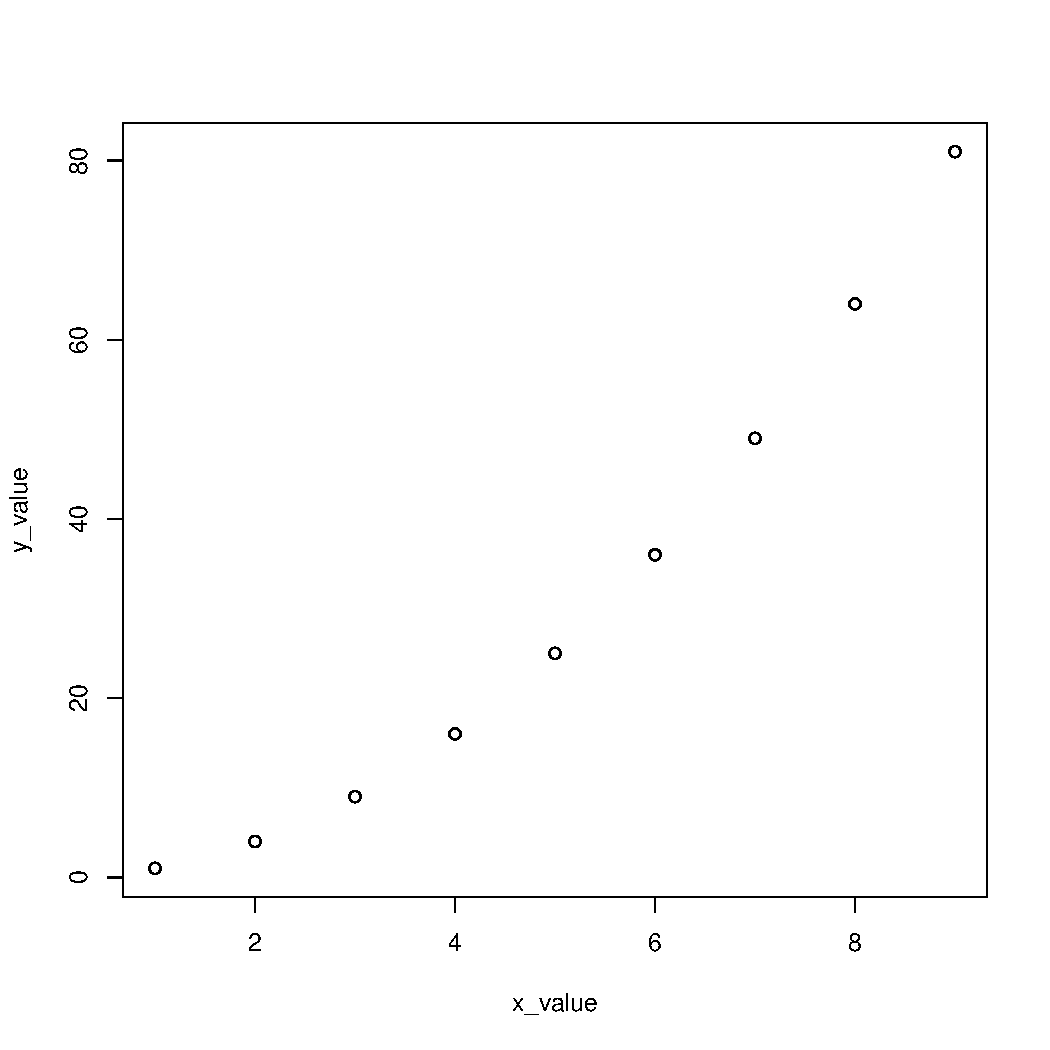
\includegraphics[width=0.5\textwidth]{diagram.pdf}
	\caption{Diagram.}
	\label{fig:diagram}
\end{figure}

\begin{figure}[t!]
	\centering
	\verbatiminput{regression-table.txt}
	\caption{Regression.}
	\label{fig:regression}
\end{figure}

This is the first sentence of my homework and has no meaning.
Anyway,
the data plot is shown in Figure \ref{fig:diagram},
the regression result is shown as Figure \ref{fig:regression}.

\end{document}
